\begin{frame}
\frametitle{Are neutrinos Majorana Particles?}

\includegraphics[scale=0.30]{img/DoubleOrNothing.png}
\end{frame}

\begin{frame}
\frametitle{Double Beta Decay}
\begin{columns}
\column{0.45\textwidth}
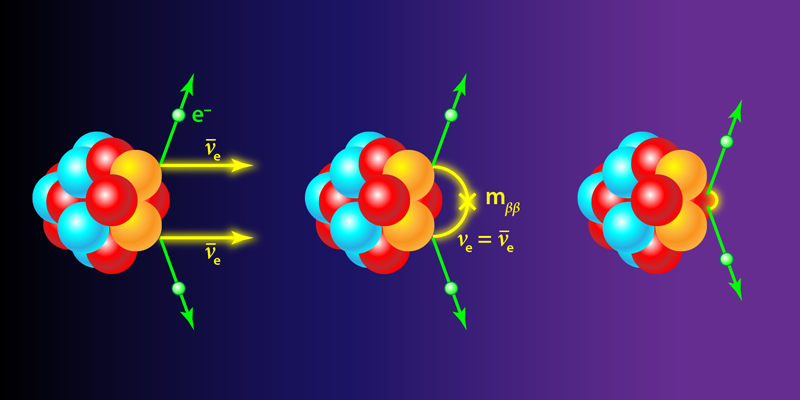
\includegraphics[scale=0.2]{img/doublebeta.png}
 
 \column{0.5\textwidth}
%\begin{block}{}
Double Beta ($\beta\beta$) decay occurs in a number of nuclear isotopes. 

The allowed process ($\beta\beta 2\nu$) is ``simply" the simultaneous decay of two neutrons. It is a very rare (long lifetime), but otherwise totally standard reaction. The lifetime of the process depends on the isotope, the order of magnitude is $10^{18}-10^{20}$ years (compare with the lifetime of the Universe, $10^{10}$ years.

The ``forbidden process" (($\beta\beta 0\nu$) occurs if and only if neutrinos are Majorana particles. The lifetime of the process depends of the neutrino masses and mixing angles. Experimentally we know that $T_0 > 10^{26}$ years. Current data suggests that $T_0 > 10^{27}$ years at least, quite likely larger. 
%\end{block}
\end{columns}
\end{frame}

\begin{frame}
\frametitle{Double Beta Decay isotopes}
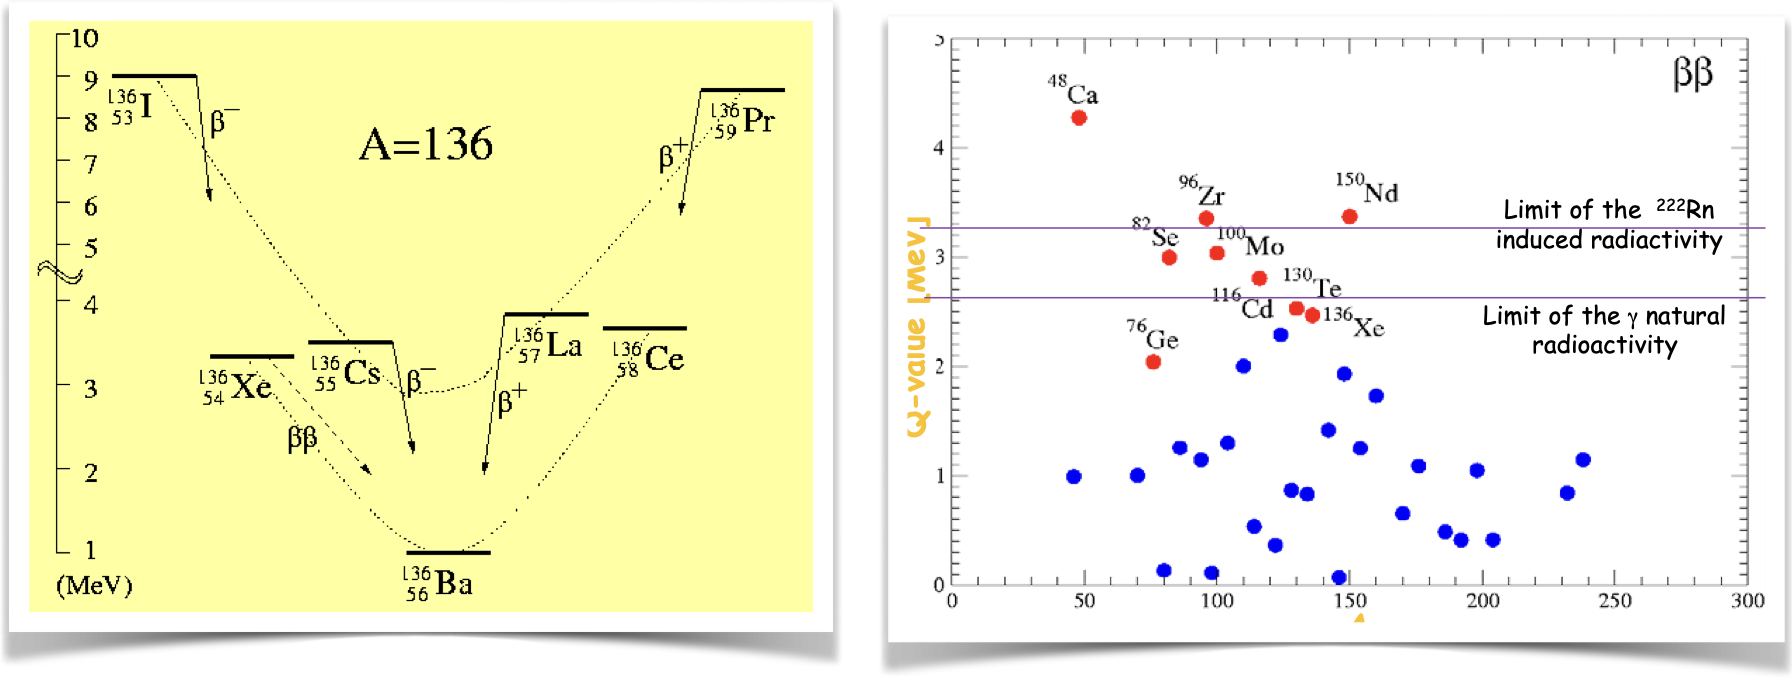
\includegraphics[scale=0.35]{img/BBIsotopes.png}
\end{frame}

\begin{frame}
\frametitle{Feynman Diagrams}
\begin{columns}
\column{0.45\textwidth}
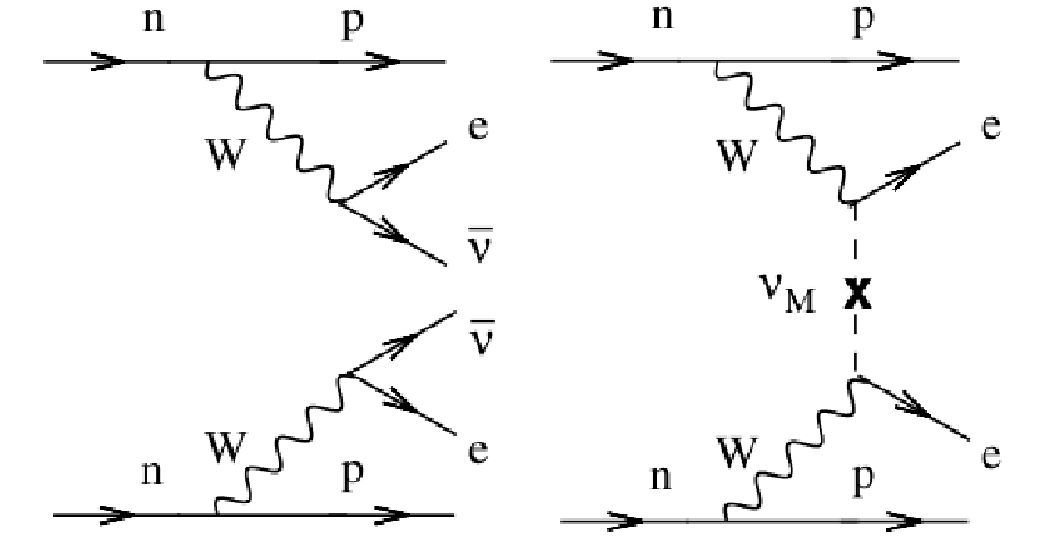
\includegraphics[scale=0.15]{img/feynman2.png}
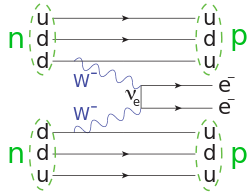
\includegraphics[scale=0.35]{img/250px-Double_beta_decay_feynman.svg.png}
 
 \column{0.5\textwidth}
%\begin{block}{}
The first diagram shows two independent neutrons emitting a W (which turns them into protons). The W, in turn, couples to and electron and a neutrino. This is simply the standard double beta decay, with a much smaller probability dictated by the fact that the two neutrons must decay simultaneously.  

The second diagram shows an alternative decay route. Here, the two W are connected by a neutrino. This requires two conditions: a) the neutrino is virtual (like the W), and b) the neutrino helicity flips between emission and absorption, so that one W emits an antineutrino and the other W absorbs a neutrino. This can only happen if the neutrino is a Majorana Particle. 
%\end{block}
\end{columns}
\end{frame}


\begin{frame}
\frametitle{A formula for $\beta\beta 0 \nu$ lifetime}

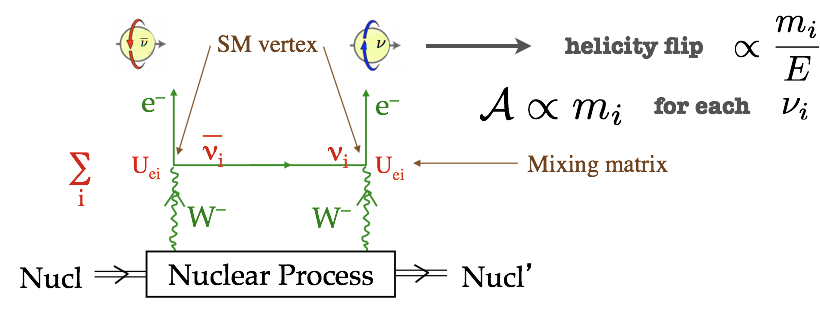
\includegraphics[scale=0.35]{img/DoubleBetaDiagram2.png}

%\begin{block}


\begin{empheq}[box=\fbox]{align}
  (T_{1/2}^{0\nu})^{-1} = G^{0\nu} |M^{0\nu}|^2 m_{\beta\beta}^2 \nonumber
\end{empheq}
%\end{block}
\end{frame}



%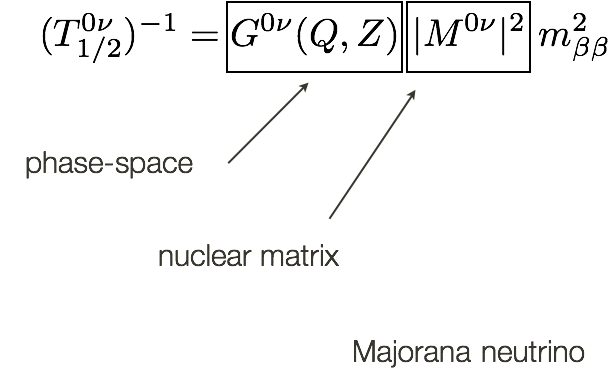
\includegraphics[scale=0.30]{DoubleBetaLifetime.png}
%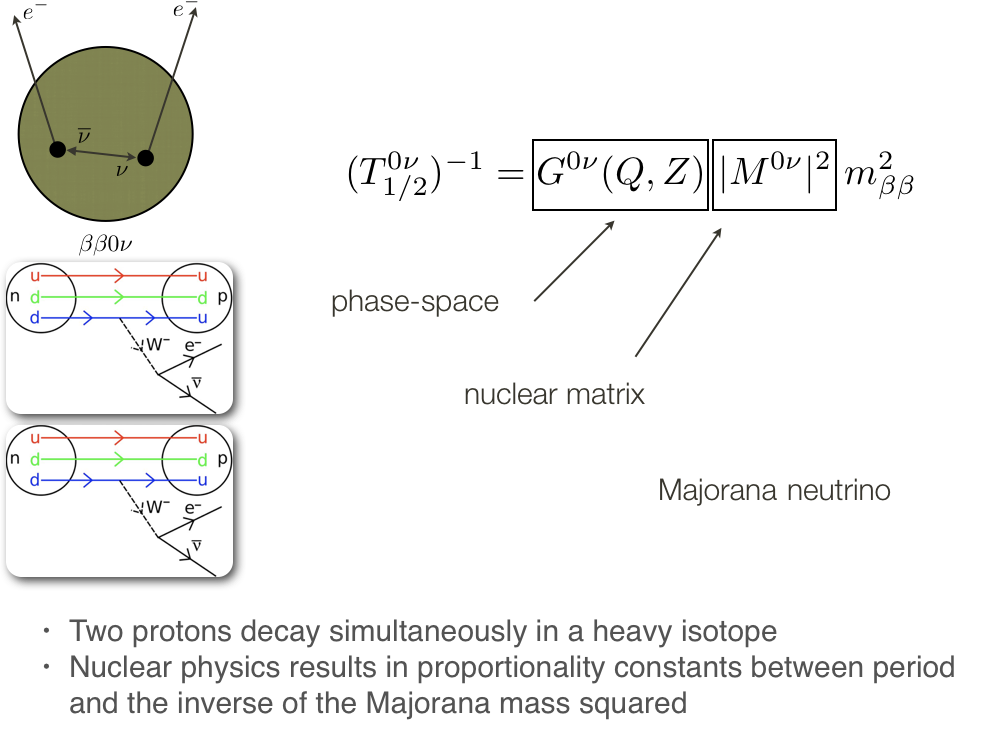
\includegraphics[scale=0.20]{img/bbmatrix.png}

\begin{frame}
\frametitle{Majorana's Lanscape}
\begin{columns}
\column{0.55\textwidth}
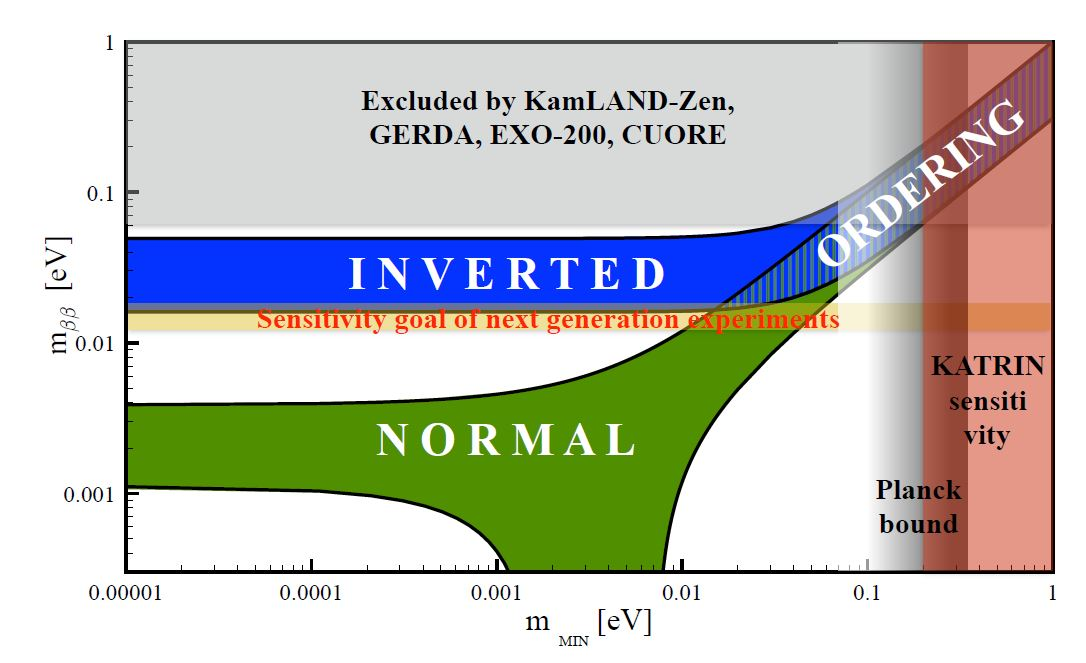
\includegraphics[scale=0.35]{img/doublebetas.jpg}
$T_{1/2}^{0\nu} \sim 10^{27}$y  $\approx m_{\beta\beta} \sim 20$meV. \alert{Explore IO}

 \column{0.45\textwidth}
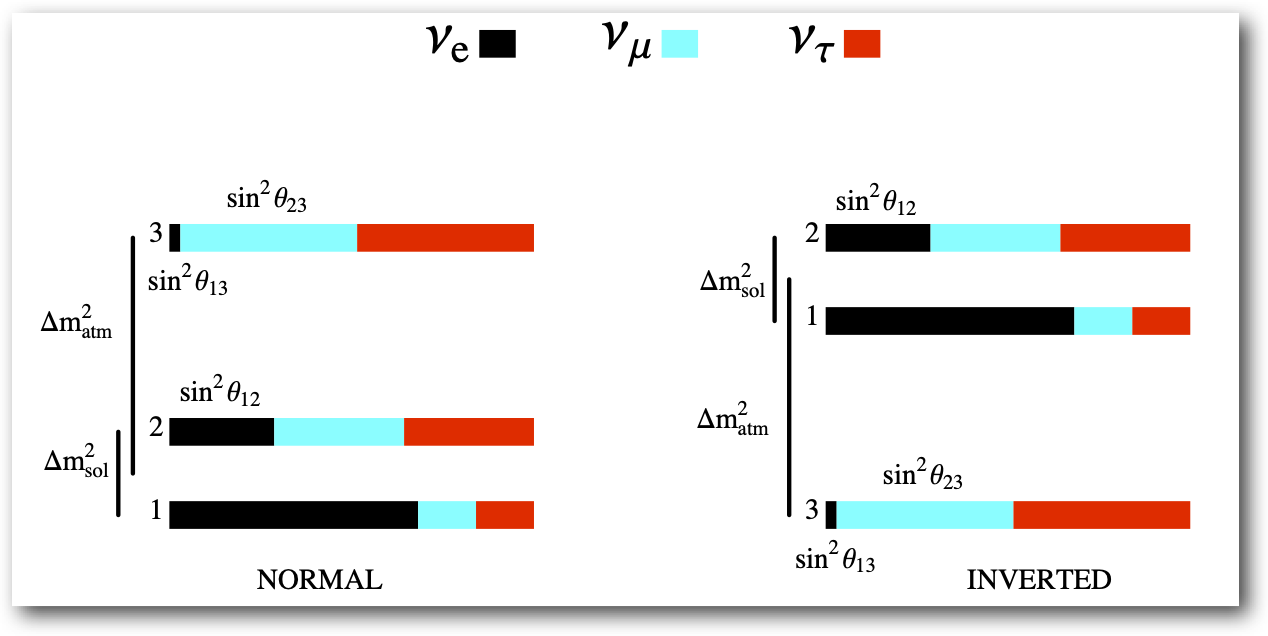
\includegraphics[scale=0.25]{img/nuhierarchies.png}
$T_{1/2}^{0\nu} \sim 10^{29}$y  $\approx m_{\beta\beta} \sim 2$meV. \alert{Explore NO}
\end{columns}


\end{frame}



\begin{frame}
\frametitle{An ideal double beta decay experiment}
\begin{columns}
\column{0.45\textwidth}
\includegraphics[scale=0.35]{img/IdealBB2.png}
\column{0.5\textwidth}
%\begin{block}{}
$\bullet$~Get yourself a detector with perfect energy resolution.

$\bullet$~Measure the energy of the emitted electrons and select those with $(T_1+T_2)/Q = 1$.

$\bullet$~Count the number of events and calculate the corresponding half-life. 

$\bullet$~In ${136}^{}Xe$, a perfect detector of 1 ton observes 3 events for a lifetime of $10^{27}$ y ($\sim$ 20 meV).

$\bullet$~Improvement in sensitivity to $m_{\beta\beta}$ goes with $\sqrt{T}$ ($\beta\beta$ tragedy number one) 
%\end{block}
\end{columns}
\end{frame}


\begin{frame}
\frametitle{Why $\beta\beta0\nu$ experiments are difficult}
\begin{columns}
\column{0.45\textwidth}
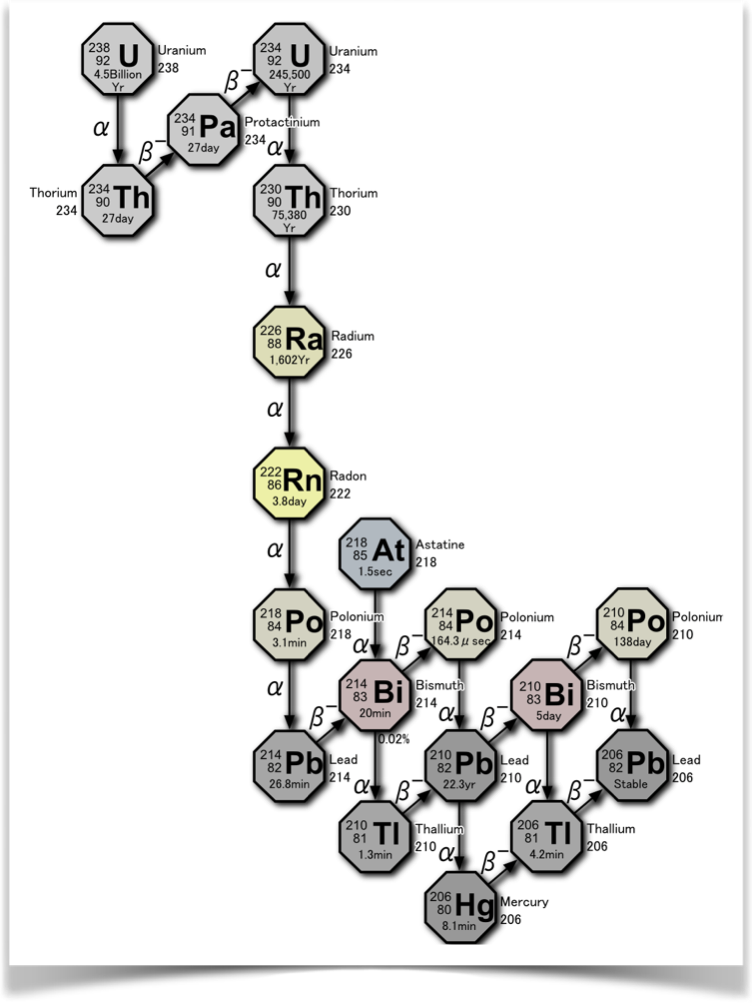
\includegraphics[scale=0.35]{img/Uchain.png}
\column{0.5\textwidth}
$\bullet$~Earth is a very radioactive planet. There are about 3 grams o ${238}^{}U$ and 9 grams of ${232}^{}Th$ per ton of rock around us.

$\bullet$~This is an intrinsic activity of the order of 60 Bq/kg of ${238}^{}U$ and  90 Bq/kg of ${232}^{}Th$.

$\bullet$~The lifetime of ${238}^{}U$ is of the order of $10^9$ y and that of ${232}^{}Th \sim 10^{10}$ y. 

$\bullet$~We want to explore lifetimes of of the order of $10^{27} -10^{29}$ y.

$\bullet$~The problem is much harder than finding a needle in a haystack 
\end{columns}
\end{frame}

\begin{frame}
\frametitle{Majorana's Beach}

\includegraphics[scale=0.30]{img/beach}

$\bullet$~Majorana’s beach: A beach with $10^{17}$ grains of sand.

$\bullet$~About $1.5 \times 10^9$ grains per square meter (to a depth of 3 m).

$\bullet$ Thus, Majorana’s beach is 70 km long and 1 km wide.

$\bullet$~Next generation $\beta\beta 0 \nu$ experiments will try to find a grain of sand in such a beach. 
\end{frame}

\begin{frame}
\frametitle{The signal and the noise}
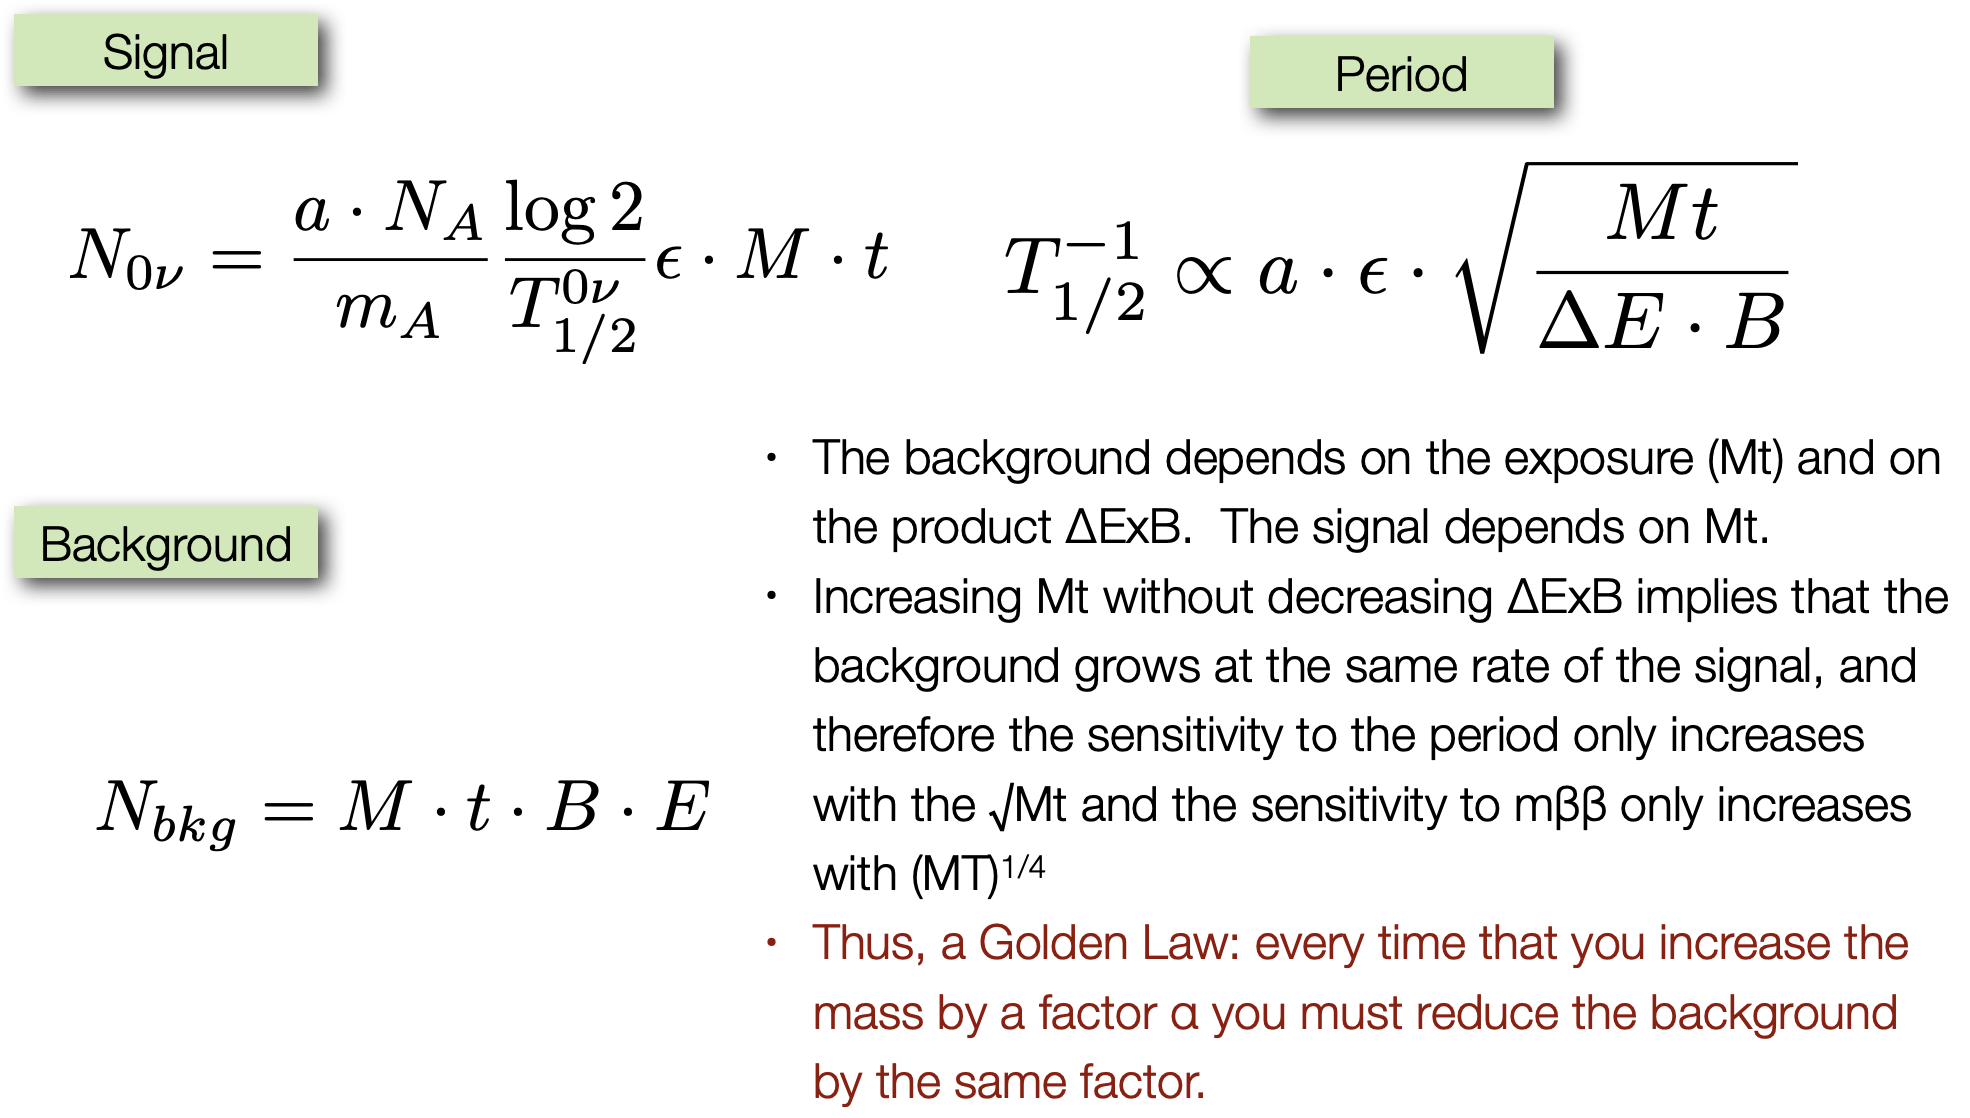
\includegraphics[scale=0.30]{img/signalAndNoise.png}
\end{frame}


\begin{frame}
\frametitle{Recipe for a $\beta \beta 0 \nu$ experiment}
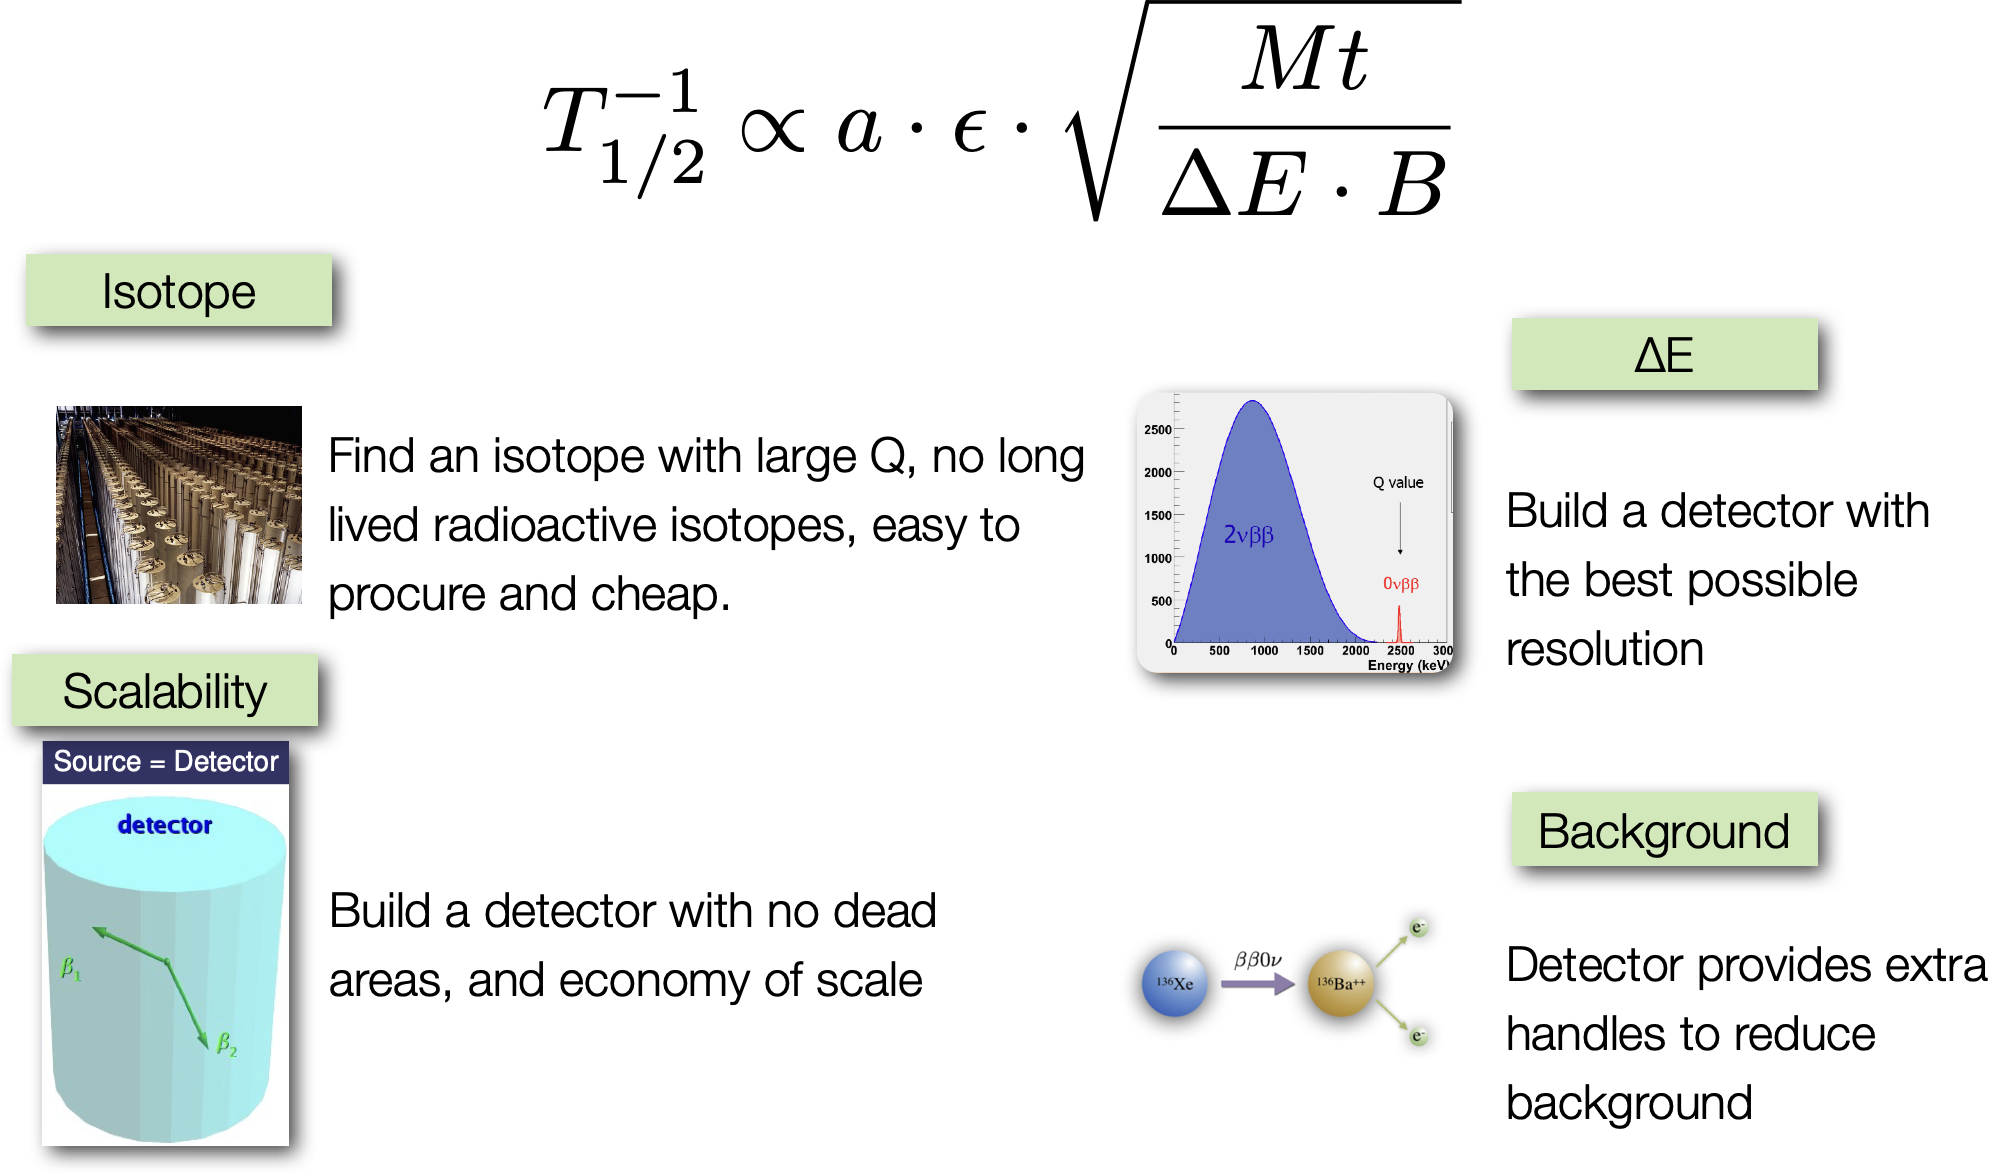
\includegraphics[scale=0.30]{img/RecipeExperiment.png}
\end{frame}


%
%
%
%
%
